\chapter{Implementation}

% - Should the subsections more or less reflect the columns in the table?

\section{Hardware Implementation}

% - EXPLAIN MORE ABOUT HARDWARE CHOISES, why these specific componens. What were the requirements for choosing these components

The first step was to evaluate what components are required for the robot to have basic navigation capabilities.
Commercially available low power components have been evaluated, where the main criteria was a low minimal supply voltage.
Currently there are only a limited amount of motor controllers on the market that can operate at the 2.0V.
To make sure that a small drop in system voltage would not create instability a margin of 0.2V was added.
Now the system voltage of 2.2V has been determined, each part of the robot will be explained in more detail. 

\subsection{Computation and Sensing}

The robot is designed around a WISP 5 \cite{wisp5_wiki_2017}, a battery-free platform for low power sensing, computation and communication.
This platform has the ability to communicate with RFID readers and is powered by the carrier signal emitted by the reader.
However, the communication range and the power that can be harvested is limited.
Therefore communication is currently not implemented and a different energy source for harvesting will be used.
Currently only the Microcontroller (MCU) is being utilized, a Texas Instruments MSP430FR5969 ultra low power microcontroller.
This MCU can operate at 16 MHz and features 64 KB FRAM, 2 KB SRAM and 40 IO ports.

The robot has access to basic sensors which can be interfaced trough I2C.
For detecting obstacles in front of the robot, a Maxim Integrated MAX44000 proximity sensor was added of the robot facing forward.
This sensor switches a IR led at high frequency to reduce the power consumed.
The same sensor is based around a photo-diode it can be used to measure the amount of ambient light as well.
To allow for controlled movements the robot has a Bosch Sensortec BMG250 low power triaxial gyroscope to measure yaw-rate, used to correct it's heading when necessary.

\subsection{Locomotion}

% tell that also higher geared motors were tried??

Two 26:1 sub-micro plastic planetary gearmotors from Pololu are mounted in a 3d printed frame.
The motors are positioned diagonally opposite from each other making the robot as compact as possible, while this differential drive configuration allows the robot to steer.
Small plastic wheels with rubber tires are mounted directly on each of the motor shafts.
Behind these two motors a free running caster wheel is mounted to the frame, acting as a third support point for the robot.

The speed of each motor can be controlled individually using Pulse-Width-Modulation (PWM) and a Texas Instruments DRV8836 dual H-bridge.
Typically MCU io-ports are limited in the amount of current that they can supply.
MOSFETs inside the dual H-bridge allow regulation of larger currents to the motors.
The MCU can use the H-bridge to enable, disable and control the direction of rotation of each individual motor.

%TODO tell something about the maximum speed that can be achieved

On average the each motor consumes 38mA while running on a flat surface, which is well within the current limit that the buck converter can supply.
However when the motors are in not moving yet the start current is approximately equal to the stall current, which is equal to 240mA.
This amount of current can not be supplied by a most regulators, PWM can be used to reduce the average current allowing a bulk capacitor to supply the voltage.

\subsection{Energy Harvesting}
\label{sec:energy_harvesting}

Solar energy is harvested from two IXYS SLMD121H04L-ND solar cells in parallel.
These monocrystalline solar cells have a high efficiency of 22\%, allowing energy harvesting even in low light conditions.
The solar cells are connected to a Texas Instruments BQ25570 energy harvester. 
This harvester includes a nanopower boost charger with maximum power point tracking to extract the optimal amount of energy from the solar panel. 
The harvested energy is stored in a 22mF - 4.5V supercapacitor from AVX, chosen for it's low leakage current and small size.
The Texas Instruments BQ25570 has a buck converter to efficiently regulate the capacitor voltage down to the system voltage of 2.2V.
External resistors can be used to program voltage thresholds, allowing to automatically enable and disable the buck converter based on minimum and maximum thresholds.
Additionally the resistors are used to set the overvoltage protection and the buck converter output voltage.

\subsection{Integration}

Now that all the parts have been chosen, they can be connected together to form the robot.
A Printed Circuit Board (PCB) has been designed to ease connection, increase stability and was required because the ICs come in small no-leads packages.
A complete overview of the robot can be found in Figure \ref{fig:robot_overview}.
Most components are part of the PCB, only the larger components are mounted externally.
Most reference designs are extendable but this adds complexity, while weight and size are the main constraints of this robot design.

% Features of the pcb, wisp regulator allows powering from battery for testing

The top of the PCB contains all the surface mount components that are soldered to the PCB using a reflow oven. 
When the boards come out of the oven, the headers, motors and supercapacitor are soldered to the boards by hand.
The PCB contains headers to connect the solar panel, a header to connect all the required pins from the WISP and a additional header to connect a battery for testing purposes.
A overview of both the top and bottom side of the PCB can be found in Figure \ref{fig:pcb_robot}.


\begin{figure}
	\centering
	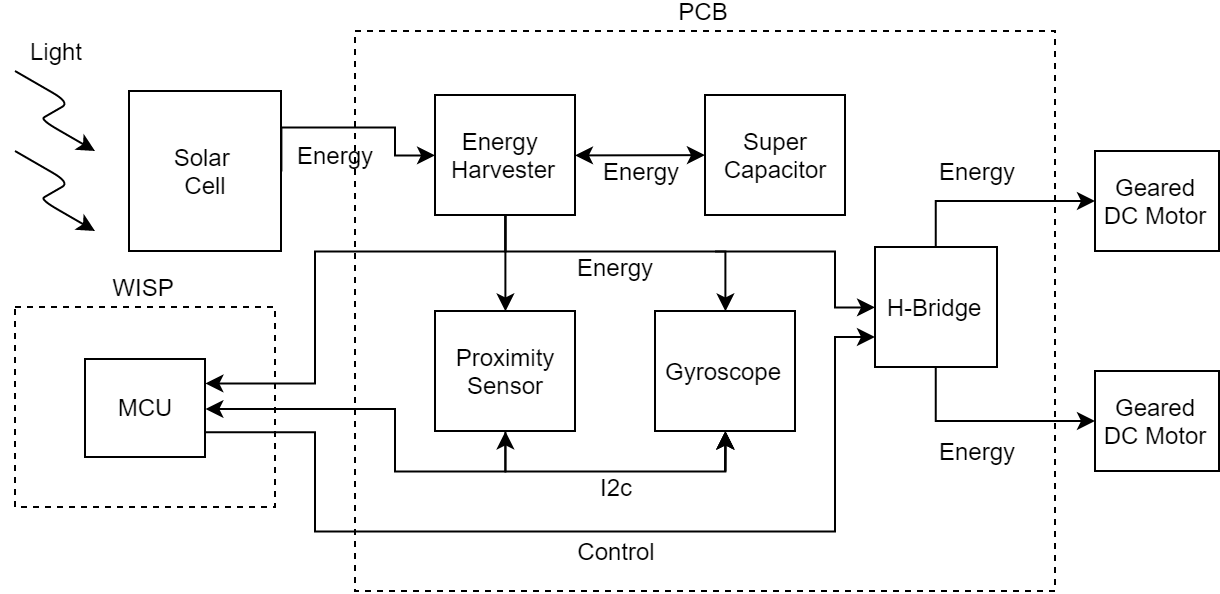
\includegraphics[width=\textwidth]{pics/schematic_robot_v2.png}
	\caption{Schematic overview of the robot}
	\label{fig:robot_overview}
\end{figure}


\begin{figure}
	\centering
	\begin{subfigure}[b]{0.45\textwidth}
		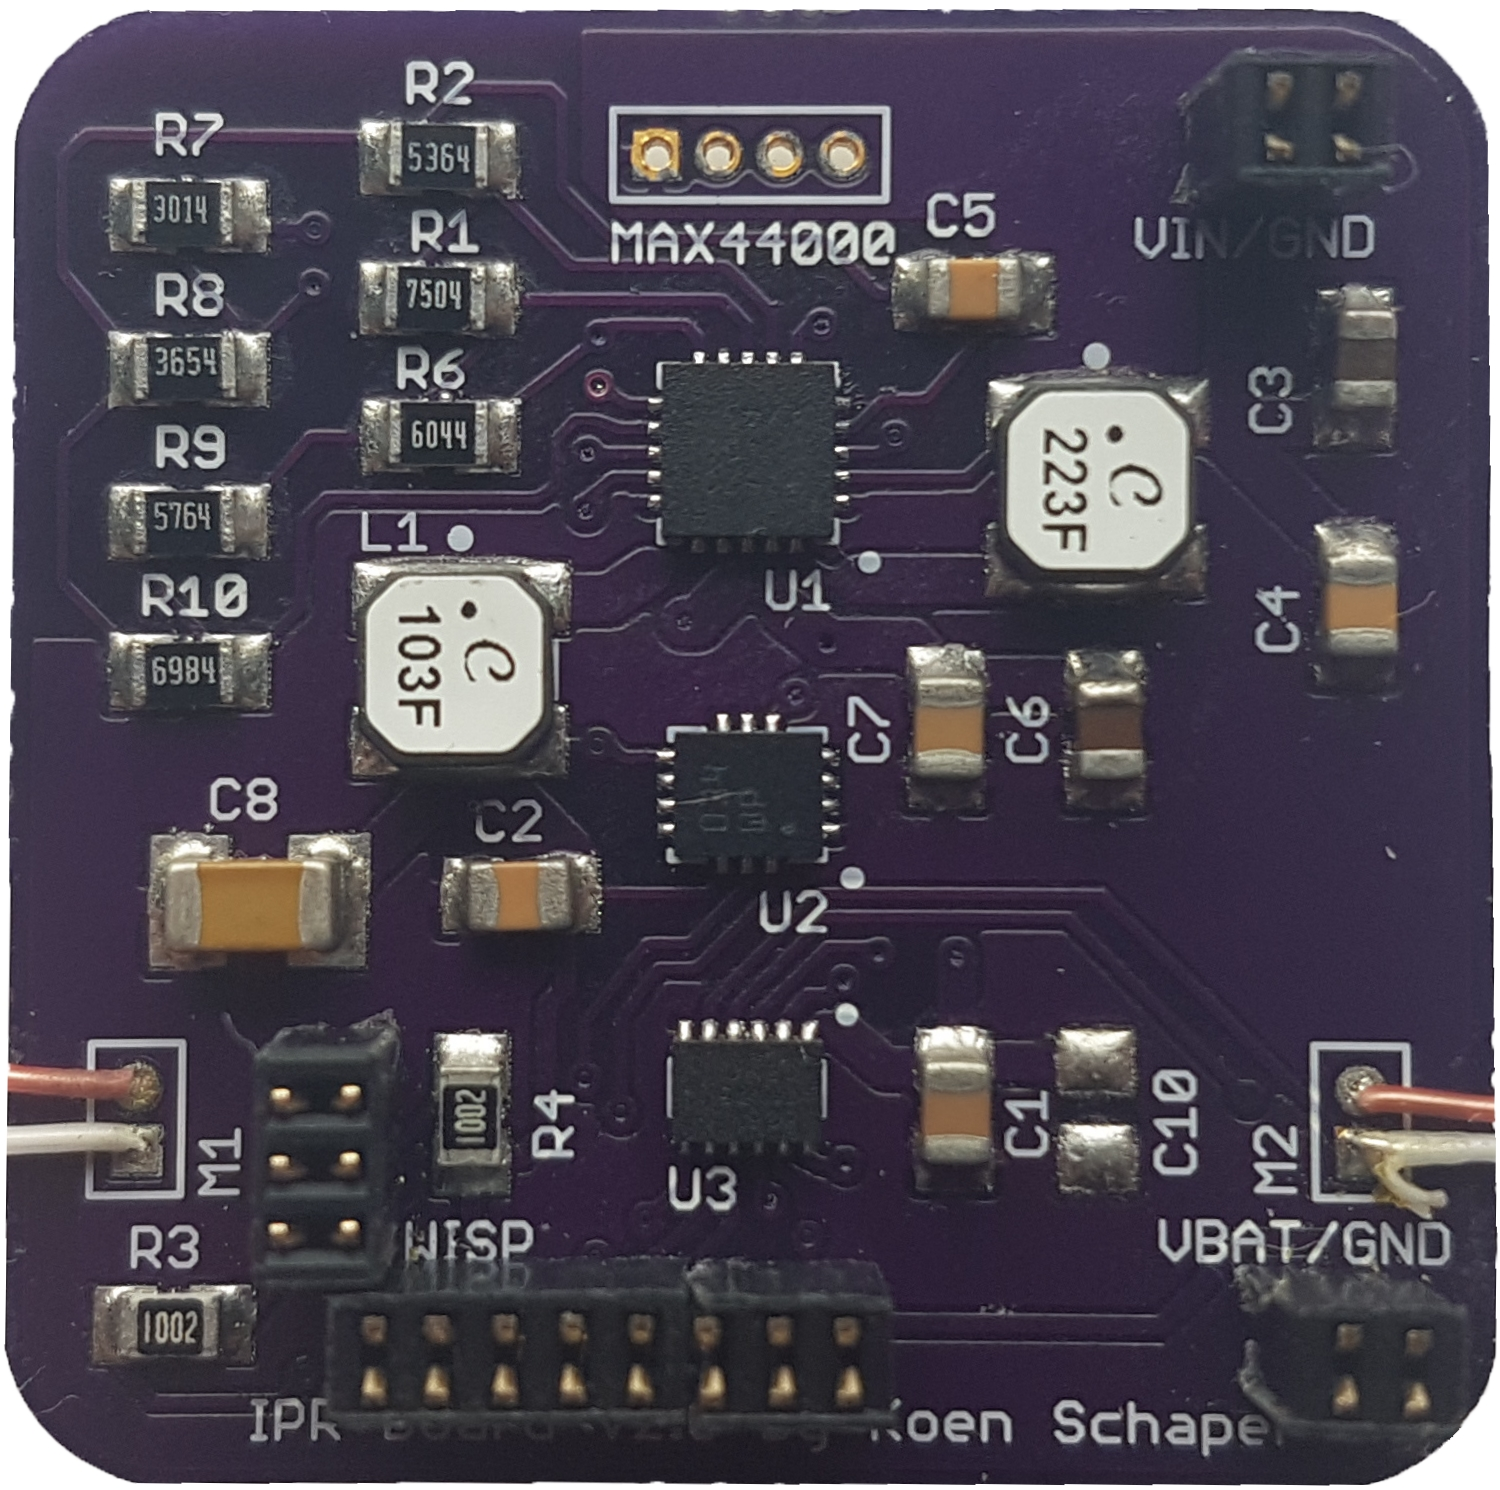
\includegraphics[width=\textwidth]{pics/pcb_front.jpg}
		\caption{Top side of the PCB}
		\label{fig:pcb_robot_front}
	\end{subfigure}
	\qquad
	\begin{subfigure}[b]{0.45\textwidth}
		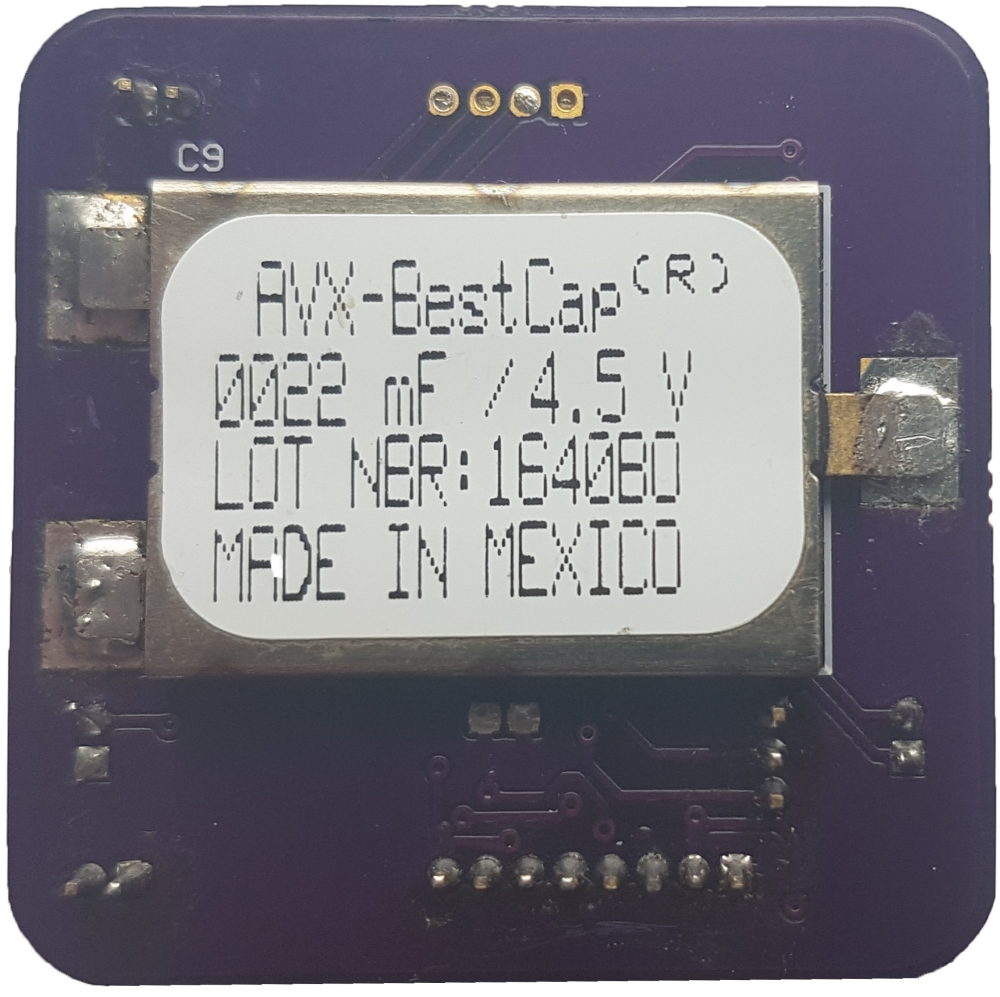
\includegraphics[width=\textwidth]{pics/pcb_back.jpg}
		\caption{Bottom side of the PCB}
		\label{fig:pcb_robot_back}
	\end{subfigure}
	\caption{The PCB designed for the robot to connect everything to the larger components}
	\label{fig:pcb_robot}
\end{figure}


The average current consumed of each component was measured with a Monsoon Power Monitor \cite{monsoon_powermonitor_2017}.
First a two second current trace was recorded of the current consumed by the microcontroller on the WISP.
The microcontroller was then used to enable each component one by one.
After enabling a two second current trace was saved.
The average of each current trace was calculated, and the current consumed by the microcontroller subtracted from the average current of each component.
The result can be found in Table \ref{tab:avg_cur_comp}.

% Make a overview of the cost to build a robot

\begin{table}[t]
	\centering
	\begin{threeparttable}
		\caption{Average consumed current for each individual component at 2.2V}
		\label{tab:avg_cur_comp}
		\begin{tabular}{|l|l|} 
			\hline
			Part & Active Current \\
			\hline\hline
			Proximity sensor & 119 \textmu A \\
			Gyroscope & 848 \textmu A\\	
			Microcontroller @ 8MHz & 522 \textmu A\\
			H-bridge & 349 \textmu A \\
			Two DC motors\textsuperscript{1} & 27--50 mA  \\
			\hline \hline
			Total & 29--52 mA \\
			\hline
		\end{tabular}
		\begin{tablenotes}
		\small
		\item [1] Current consumed varies per motor and motor speed
		\end{tablenotes}
	\end{threeparttable}
\end{table}

Cost of a single robot to build excluding MCU :

\begin{table}[t]
	\centering
	\caption{Cost per robot to build 20 or more}
	\label{tab:cost_robot}
	\begin{tabular}{|l|l|} 
		\hline
		Part & Price \\
		\hline\hline
		Solar panel & \euro9,60\\
		Supercapacitor & \euro7,43\\
		Harvester & \euro5,48 \\
		Proximity sensor & \euro3,98 \\
		Gyroscope & \euro2,81\\	
		H-bridge & \euro1,47 \\
		Two DC motors & \euro18,51 \\
		Wheels & \euro3,08\\
		PCB & \euro2,50 \\
		Small components & \euro4,53\\
		\hline \hline
		Total & \euro59,39 \\
		\hline
	\end{tabular}
\end{table}


\section{Software Implementation}

\subsection{Calibration of the Motors}
\label{sec:calib_motors}

%TODO STIL VALID? (Write about why valid to assume a constant speed on a single surface)
The motors used for robots are powered directly from the battery as linear or switch-mode power regulators are not able to supply the high start-up currents.
When the motors are powered from the battery the supplied voltages drops while energy is consumed for the battery.
Since the speed of the motor is dependent on the supply voltage the speed of the motor will also decrease while energy is consumed from the battery.
However, the use of a supercapacitor requires a regulator to make efficient use of the energy stored, as described in Section \ref{sec:energy_harvesting}.
A benefit of keeping the supply voltage constant is that voltage is eliminated as a factor in determining the motor speed.
By making the assumption that the robot will only travel on a flat surface, the steady state speed is considered "constant" given a certain PWM duty cycle.


\subsubsection{PWM Frequency for linear Motion Control}
% Write about linear motion control dc motor vs pwm
% Reference: https://www.precisionmicrodrives.com/application-notes/ab-022-pwm-frequency-for-linear-motion-control

Pulse width modulation(PWM) is used to control the speed of the motors, the average current supplied to the motors can be regulated by changing the duty cycle.
When the motor is at rest it's equivalent circuit consists of a resistance and inductance in series.
When voltage is applied to the motor the rate at which the current rises is limited by the inductance. 
All RL circuits have a time constant: $\tau = L / R$ and the current reaches it's maximum steady state at $5\tau$. 
The motors used for the robot have a typical resistance R of 14.5 Ohm and an inductance of 70 $\mu$L~\cite{gearmotor_206-110_2017}.
Therefore the minimum pulse width should be equal to:

\begin{equation}
	5\tau = 5 \frac{L}{R} 
\end{equation}

From this can be calculated that the minimum pulse width should be $5\tau = 5 \cdot \frac{70 \cdot 10^{-6}}{14.5} = 24.14 \mu s $
If a minimum pulse width of is assumed, than the maximum PWM frequency becomes:

\begin{equation}
	f_{max} = \frac{t_{on}}{5\tau \cdot 100 }
\end{equation}

If the PWM frequency is assumed to be at least 5\% than the maximum PWM frequency is equal to $\frac{5}{24.14 \cdot 100} = 2071.25 Hz$.
The PWM frequency will be set to 2kHz and later will be verified that the duty cycle will never go below the minimum of 5\%.

% -Write how the pwm control signals are generated for the H-bridge. 
The PWM signals are generated by the microcontroller on the WISP.
Four io-ports are available on the WISP which can be directly controlled by a single timer.
The timer is configured to use a compare register for each of the ports.
When the timer reaches a value that corresponds to a value one of the compare registers the connected port is toggled automatically.
This way the overhead is minimized because no interrupt service routine is required.

\subsubsection{Minimal Duty Cycle}

The minimal PWM duty cycle to produce a torque that is able to overcome the static friction between the wheels and a surface the robot is moving on.
Each motor is physically different and the friction in the gearbox can variate as well, which results in a variating output speeds per motor.
Since the robot uses two motors in differential drive configuration, a minimum PWM duty cycle has to be found for each motor.
This is accomplished by setting a PWM duty cycle at which both motors are rotating and slowly backing down the PWM duty cycle until one or both stop turning.
The minimum PWM duty cycle, allowing the wheels to rotate, is stored as a calibration and added to every motor set point.
If the robot is set to run at the minimum speed does not mean that the motors run at the same speed.

\subsubsection{Maximal Duty Cycle}
% -Write about maximum speed due to enabling two motors and their startup current peak! show figure!!
% Does more gearing (more torque) reduce the current peak??

The maximum PWM duty cycle is bounded by the amount of current that the buck converter and bulk capacitor can supply.
The back electromotive force (back EMF) of a dc motor at rest is equal to zero.
When voltage is applied to the motor, current rises as quickly as the inductance in the motor windings allows. 
The current peaks when the rotor starts to rotate and a back EMF is generated.
The back EMF will further increase while the motor accelerates to it's steady state speed, and the speed is limited by the voltage supplied.
Lowering the PWM duty cycle reduces both the maximum current peak and the steady state current and therefore can be used to reduce the motor start current demand.
The maximum PWM duty cycle can be found by increasing the duty cycle until the robot is not able to start a movement from that PWM set point. 

\subsection{Closed loop feedback for controlled movements}

The robot uses two physically different motors in differential drive configuration which are mounted in a non-symmetrical way.
Open loop movement using just a calibrated motor values has been used in previous work \cite{legoc_uist_2016}, but it can be time consuming and any little disturbance will trow the robot off course.
The gyroscope is used to obtain the current yaw-rate and correct the robots heading.
Controlled movements are possible using closed loop feedback, where the heading is used to update the motor control values.

The robot can be controlled using three different commands, one for straight trajectories, one for left and one for right turns.
When a command is executed a control loop will run until the provided target is reached.
A timer running periodically calling a interrupt service routine which executes the control loop.   
Each command requires different initial values, set points and tuning parameters, these are set accordingly before the control loop is enabled.

\subsubsection{Controlled straight trajectories}

% -Why pid for straight movements and not a simple p controller?
% --Fast reaction on disturbances without osccilation??
%TODO -Write about bounding the pid output, because otherwise the motors of the robot could stall, if the motor setpoint is to high

The control loop for straight trajectories obtains the yaw-rate from the gyroscope and uses this as an input for the Proportional–Integral–Derivative (PID) controller.
The PID will try to reduce the error and force the yaw-rate to zero for a given target motor speed.
% $ e(t) = 0 - yaw(t)$
Using the output of the PID controller the target motor speed of each motor is adjusted in opposite direction.
The loop will stop automatically when the required target is reached.
%TODO Explain that the target distance is with a calibrated value.

\begin{equation}
output(t) = K_{p}e(t) + K_{i} \int_{0}^{t}e(\tau)d\tau + Kd\frac{d}{dt}e(t) [rad/s]
\end{equation}

\subsubsection{PID tuning using Ziegler-Nichols method}

%TODO -Write about tuning the pid controller using Ziegler–Nichols tuning method (method 2), closed loop, Critical gain.

A PID loop can be tuned using three different tunable gains ($K_{p}$, $K_{i}$, $K_{d}$).
Tuning can be done trough a trail and error approach but a faster way of tuning is to use the Zigeler-Nicholos method.
The second or ultimate gain method starts with increasing or decreasing Kp until constant oscillation occurs.
From Figure \ref{fig:ultimate_gain} can be seen how the proportional gain was increased until eventually the robot started to oscillate.
With a proportional gain of 0.13 the robot starts light oscillation at the end, but this is not always the case and can be a result of the surface the robot was driving on.
% Tell something about how the right values are determined
To reduce the oscillation a $T_{u}$ of 0.2 was added as can be determined from Figure \ref{fig:gain_tuning}.
From this figure can be seen that the robot is more stable and doesn't have the tendency to oscillate anymore.
%Robots was driving on surface that was not super flat, therefore the gyro signal is noisy.
The tuning process was sped up by setting the minimum motor duty cycle as it made the robot a lot more responsive, this was described earlier in Section \ref{sec:calib_motors}.

%TODO -Add figure with critcial gain + mark period Tu

\begin{figure}
	\begin{subfigure}[b]{0.49\textwidth}
		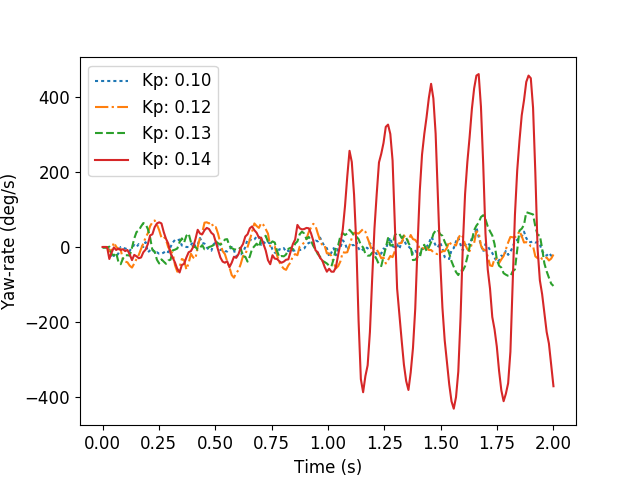
\includegraphics[width=\textwidth]{pics/straight_ku.png}
		\caption{Increase Ku until oscillation}
		\label{fig:ultimate_gain}
	\end{subfigure}
	\begin{subfigure}[b]{0.49\textwidth}
		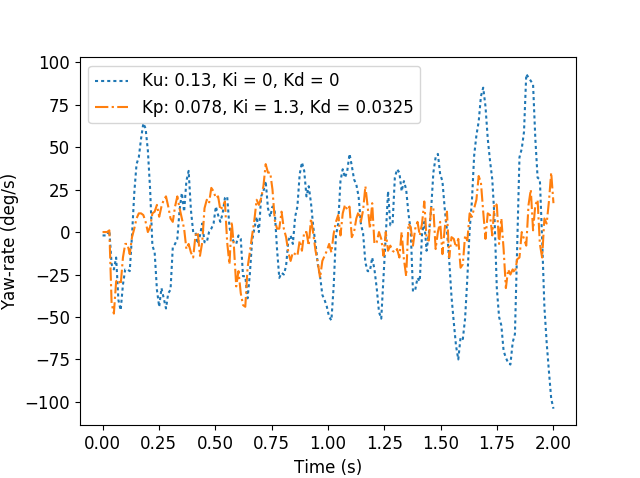
\includegraphics[width=\textwidth]{pics/straight_ku_with_tu.png}
		\caption{Find period}
		\label{fig:gain_tuning}
	\end{subfigure}
	\caption{Tuning the PID controller using the ultimate gain method}
\end{figure}

\subsubsection{Controlled curved movements} 

The same PID control loop can be used to command the robot to make curved movements.
Instead of an angular velocity set point of zero, an turn rate needs to be specified.
This desired angular velocity can be a determined from the radius of the circle that the robot needs to turn and the calibrated target speed.
By integrating the angular velocity an angle estimate is obtained, which is used to verify if the angle target given is reached within 2 degrees.
In case this is true the loop will exit automatically.

\subsubsection{Controlled turns}

The control loop for controlled turning uses the angle, which is obtained by integrating the yaw-rate sensor data from the gyroscope.
A P controller is used to rotate the robot to the desired angle, the proportional gain is directly influencing turn speed of the robot.
The motor control values are set to run the motors opposite directions and are equal to the output of the P controller.
These values will keep decreasing until the robot rotates to the desired angle.
The set point is assumed to be reached when the angle is within two degrees of the target, in this case the loop will stop automatically.
To allow enough precision to measure if the target is within these two degrees, the timer which executes the control loop was set to run at 100Hz.
Secondly, the proportional gain should not be set to low because it can happen that the robot is not able to reach the target but also not to high as it can overshoot the target.

\subsection{Persistent movement}

Normally when a robot is battery powered, it can execute some predefined movements and stop when required.
In case of the transiently powered robot one movement or a series of movements is likely to require multiple power cycles to complete.
To be able to finish a movement and not reset i.e. redo the same movement over and over, a simple check pointing method is used to keep the program state across power cycles.
A persistent counter registers the progress in the set of movements.
In the control loop only the progress in moving towards a set point is stored in non-volatile FRAM memory, which depending on the movement can be a required time or angle.
The right and left motor speed which are tuned by the controllers are not saved and restored after a power interrupt.
The motors have a startup phase the controller needs to react differently compared to the steady state, constant speed movement of the robot. 